\documentclass[12pt,oneside]{report}

%%% ========================================================================= %%%
%%% UCSF DISSERTATION MASTER LATEX TEMPLATE                                   %%%
%%% Fully compliant with UCSF Dissertation Rubric (Rev 04/24)                 %%%
%%% ========================================================================= %%%

%%% ------------ I. MARGINS, FONT & SPACING (RUBRIC SEC I.A, I.B, I.F) ------------ %%%
\usepackage[letterpaper, top=1in, bottom=1in, left=1in, right=1in]{geometry}
\usepackage{mathptmx} % Times New Roman 12pt TrueType font
\usepackage{setspace}

% Unicode symbols common in biomedical text and Crossref titles (e.g., TGF-β, ≥ 0.5).
% pdfLaTeX cannot print these on its own; map them to math symbols.
\usepackage{newunicodechar}
\newunicodechar{α}{\ensuremath{\alpha}}
\newunicodechar{β}{\ensuremath{\beta}}
\newunicodechar{γ}{\ensuremath{\gamma}}
\newunicodechar{δ}{\ensuremath{\delta}}
\newunicodechar{ε}{\ensuremath{\epsilon}}
\newunicodechar{ζ}{\ensuremath{\zeta}}
\newunicodechar{η}{\ensuremath{\eta}}
\newunicodechar{θ}{\ensuremath{\theta}}
\newunicodechar{ι}{\ensuremath{\iota}}
\newunicodechar{κ}{\ensuremath{\kappa}}
\newunicodechar{λ}{\ensuremath{\lambda}}
\newunicodechar{μ}{\ensuremath{\mu}}
\newunicodechar{ν}{\ensuremath{\nu}}
\newunicodechar{ξ}{\ensuremath{\xi}}
\newunicodechar{π}{\ensuremath{\pi}}
\newunicodechar{ρ}{\ensuremath{\rho}}
\newunicodechar{σ}{\ensuremath{\sigma}}
\newunicodechar{τ}{\ensuremath{\tau}}
\newunicodechar{υ}{\ensuremath{\upsilon}}
\newunicodechar{φ}{\ensuremath{\phi}}
\newunicodechar{χ}{\ensuremath{\chi}}
\newunicodechar{ψ}{\ensuremath{\psi}}
\newunicodechar{ω}{\ensuremath{\omega}}
\newunicodechar{Γ}{\ensuremath{\Gamma}}
\newunicodechar{Δ}{\ensuremath{\Delta}}
\newunicodechar{Θ}{\ensuremath{\Theta}}
\newunicodechar{Λ}{\ensuremath{\Lambda}}
\newunicodechar{Ξ}{\ensuremath{\Xi}}
\newunicodechar{Π}{\ensuremath{\Pi}}
\newunicodechar{Σ}{\ensuremath{\Sigma}}
\newunicodechar{Υ}{\ensuremath{\Upsilon}}
\newunicodechar{Φ}{\ensuremath{\Phi}}
\newunicodechar{Ψ}{\ensuremath{\Psi}}
\newunicodechar{Ω}{\ensuremath{\Omega}}
\newunicodechar{µ}{\ensuremath{\mu}}
\newunicodechar{≤}{\ensuremath{\leq}}
\newunicodechar{≥}{\ensuremath{\geq}}
\newunicodechar{∼}{\ensuremath{\sim}}
\newunicodechar{≈}{\ensuremath{\approx}}
\doublespacing % Double spacing throughout text

\usepackage{graphicx}
\usepackage{amsmath,amssymb,amsfonts}
\usepackage{booktabs}
\usepackage{multirow}
\usepackage{array}
\usepackage{pdfpages}
\usepackage[colorlinks=true, linkcolor=black, citecolor=black, urlcolor=black, breaklinks=true]{hyperref}
\usepackage[capitalise, noabbrev, nameinlink]{cleveref}

%%% ------------ CITATION FORMATTING (RUBRIC SEC I.H) ------------ %%%
% Consistent square brackets [1], numeric-comp style, no subscripts
\usepackage[
  sorting=none,
  backend=biber,
  style=numeric-comp,
  natbib=true,
  doi=true,
  url=false,
  isbn=false
]{biblatex}
\addbibresource{references.bib}

%%% ------------ WIDOWS & ORPHANS (RUBRIC SEC I.L) ------------ %%%
\clubpenalty=10000
\widowpenalty=10000
\displaywidowpenalty=10000

%%% ------------ HEADING HIERARCHY (RUBRIC SEC III.J) ------------ %%%
\usepackage{titlesec}

% Primary: All caps, bold, centered, double spaced above section
\titleformat{\chapter}[display]
  {\normalfont\bfseries\centering\LARGE}
  {\MakeUppercase{\chaptertitlename\ \thechapter}}
  {10pt}
  {\MakeUppercase}
\titlespacing*{\chapter}{0pt}{0pt}{30pt}

% Secondary: Sentence case, bold, left-aligned
\titleformat{\section}
  {\normalfont\bfseries\large\raggedright}
  {\thesection}
  {1em}
  {}
\titlespacing*{\section}{0pt}{18pt}{6pt}

% Tertiary: Sentence case, italic, left-aligned
\titleformat{\subsection}
  {\normalfont\itshape\large\raggedright}
  {\thesubsection}
  {1em}
  {}
\titlespacing*{\subsection}{0pt}{12pt}{4pt}

% Quaternary: Sentence case, italic, left-aligned, run-in with period
\titleformat{\subsubsection}[runin]
  {\normalfont\itshape}
  {\thesubsubsection}
  {1em}
  {}
  [.]
\titlespacing*{\subsubsection}{0pt}{6pt}{6pt}

%%% ------------ CAPTION FORMATTING (RUBRIC SEC III.A & III.B) ------------ %%%
% Table captions ABOVE, Figure captions BELOW; single-spaced with bold labels
\usepackage[labelfont=bf, textfont=normalfont, singlelinecheck=off, font={small,singlespacing}]{caption}
\captionsetup[table]{position=above, skip=6pt, font={small,singlespacing}}
\captionsetup[figure]{position=below, skip=6pt, font={small,singlespacing}}

%%% ------------ BLOCK QUOTATIONS (RUBRIC SEC I.F & III.C) ------------ %%%
% Single-spaced, indented 5 spaces from left margin
\usepackage{etoolbox}
\AtBeginEnvironment{quotation}{\singlespacing}
\AtBeginEnvironment{quote}{\singlespacing}

%%% ------------ ALL CAPS COMPONENT HEADINGS (RUBRIC SEC III.E, III.F, III.G) ------------ %%%
\renewcommand{\contentsname}{TABLE OF CONTENTS}
\renewcommand{\listfigurename}{LIST OF FIGURES}
\renewcommand{\listtablename}{LIST OF TABLES}

%%% ------------ PAGINATION & FOOTER (RUBRIC SEC I.B.2 & I.H) ------------ %%%
\usepackage{fancyhdr}
\pagestyle{fancy}
\fancyhf{}
\cfoot{\thepage} % Bottom center pagination
\renewcommand{\headrulewidth}{0pt}
\setlength{\footskip}{0.6in} % Footer distance >= 0.5in from edge

\begin{document}

%%% ========================================================================= %%%
%%% PRELIMINARY PAGES (Numbered in lowercase Roman numerals)                   %%%
%%% ========================================================================= %%%
\pagenumbering{roman}

% --- TITLE PAGE (Page i, unnumbered, Rubric Sec I.G) ---
% Note: Use the official UCSF title page PDF template signed via DocuSign
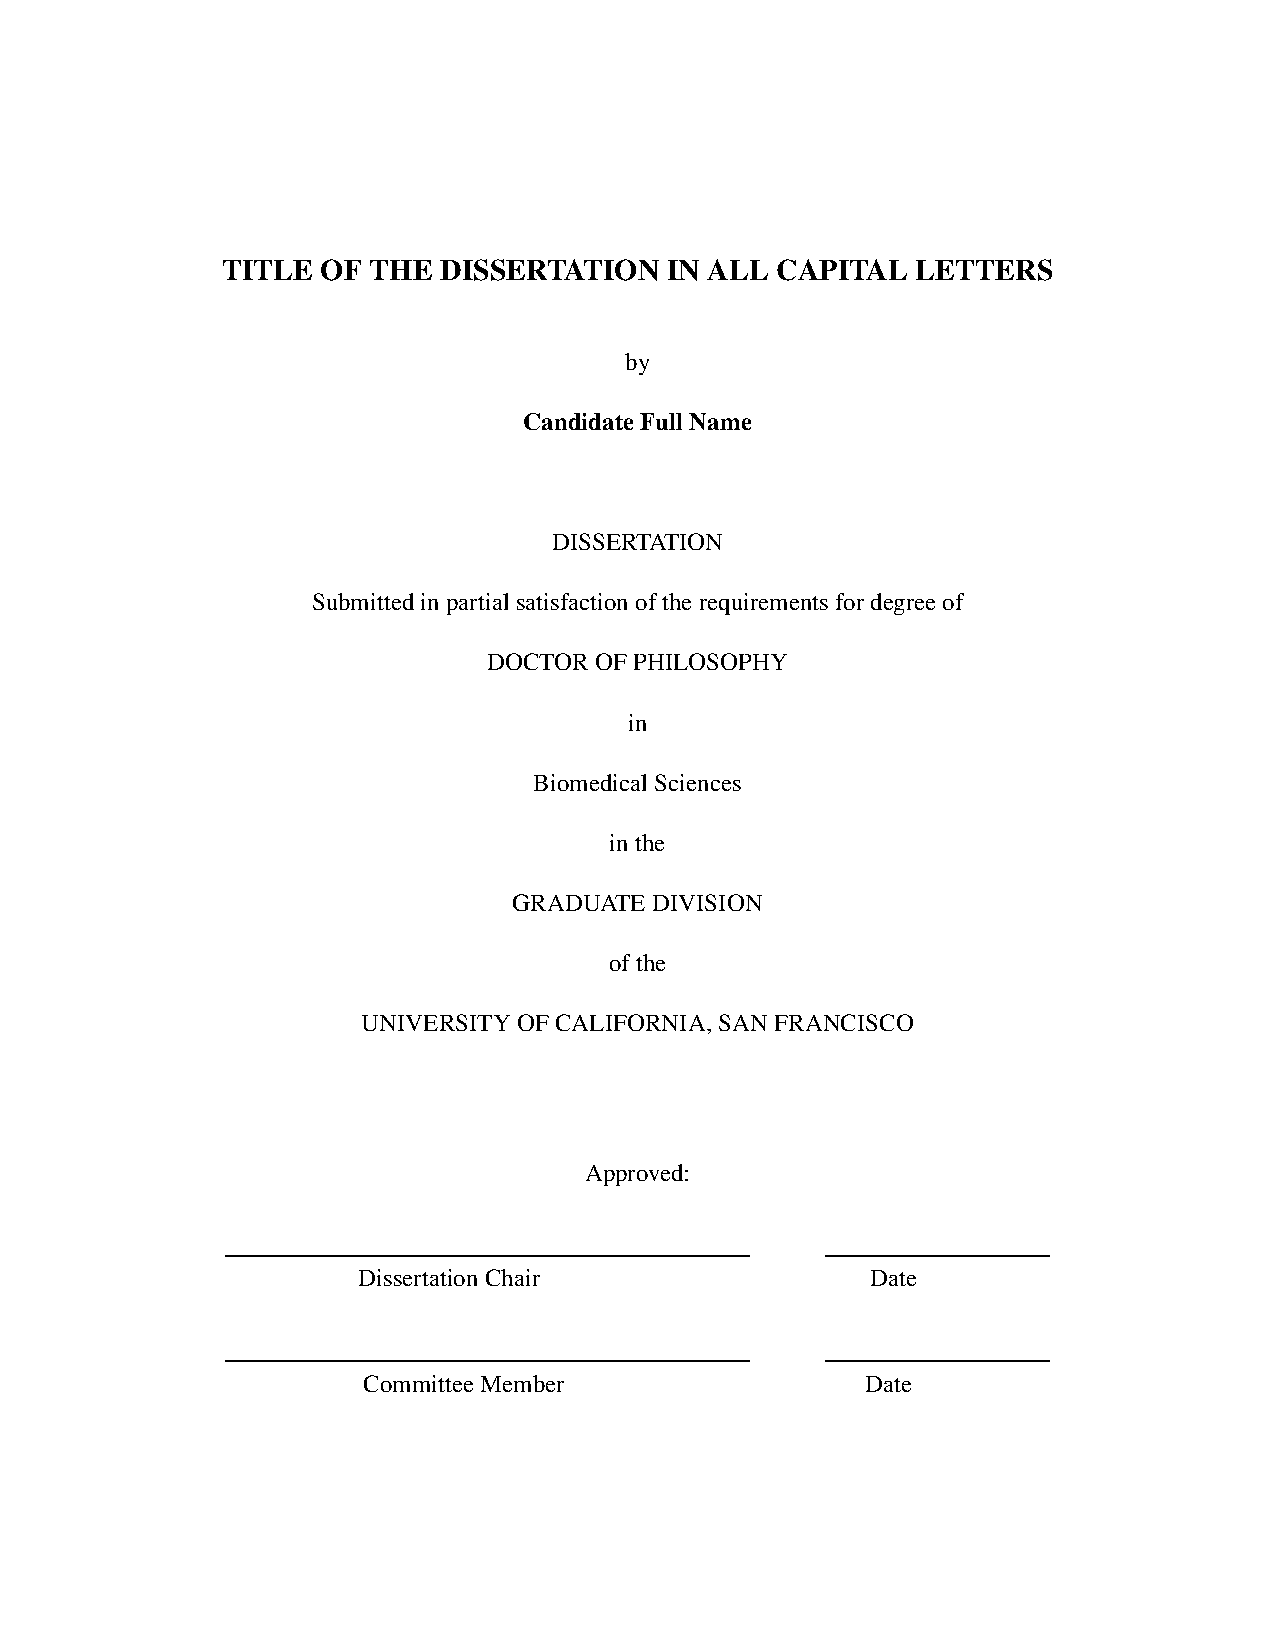
\includepdf[pages={1}]{Title_Page.pdf}
\setcounter{page}{2} % Copyright page is Page ii

% --- COPYRIGHT PAGE (Page ii, Rubric Sec I.I & III.B) ---
% Format: Copyright 20XX / by / Student Name / ALL RIGHTS RESERVED (no (c) symbol)
\thispagestyle{fancy}
\begin{center}
  \vspace*{2.5in}
  Copyright 2026\\[0.2in]
  by\\[0.2in]
  AUTHOR FULL NAME\\[0.2in]
  ALL RIGHTS RESERVED
\end{center}
\clearpage

% --- DEDICATION (Optional, Rubric Sec III.C) ---
\chapter*{DEDICATION}
\doublespacing
Dedicated to my mentors, colleagues, family, and friends who supported this journey.
\clearpage

% --- ACKNOWLEDGEMENTS (Optional, Rubric Sec III.C) ---
\chapter*{ACKNOWLEDGEMENTS}
\doublespacing
I express my deepest gratitude to my advisor, dissertation committee members, and laboratory colleagues.
\clearpage

% --- CONTRIBUTIONS (Optional, Rubric Sec III.C) ---
\chapter*{CONTRIBUTIONS}
\doublespacing
Descriptions of student and co-author contributions for adapted manuscript chapters.
\clearpage

% --- EPIGRAPH (Optional, Rubric Sec III.C) ---
\chapter*{EPIGRAPH}
\doublespacing
\vspace*{1.5in}
\begin{quotation}
  \itshape
  ``Equipped with his five senses, man explores the universe around him and calls the adventure Science.''
\end{quotation}
\begin{flushright}
  --- Edwin Powell Hubble (1948)
\end{flushright}
\clearpage

% --- ABSTRACT (Required, Rubric Sec I.N & III.D) ---
% Always appears directly before TOC; ALL CAPS Title, Name, and ABSTRACT
\chapter*{ABSTRACT}
\doublespacing
\begin{center}
  \textbf{TITLE OF THE DISSERTATION IN ALL CAPITAL LETTERS}\\[0.08in]
  \textbf{AUTHOR FULL NAME IN ALL CAPITAL LETTERS}
\end{center}
\vspace{0.05in}

\noindent A concise synthesis of the research problem, methodology, findings, and conclusions. The abstract must be double-spaced and contain no abbreviations in the title.
\clearpage

% --- TABLE OF CONTENTS (Required, Rubric Sec III.E) ---
% Excludes preliminary pages and publishing agreement; ALL CAPS centered title
\tableofcontents
\clearpage

% --- LIST OF FIGURES (Required if figures present, Rubric Sec III.G) ---
% On its own page, separate from List of Tables
\listoffigures
\clearpage

% --- LIST OF TABLES (Required if tables present, Rubric Sec III.F) ---
% On its own page, separate from List of Figures
\listoftables
\clearpage

% --- LIST OF ABBREVIATIONS (Required if abbreviations used, Rubric Sec I.P & III.H) ---
\chapter*{LIST OF ABBREVIATIONS}
\doublespacing
\begin{tabular}{lp{5in}}
  \textbf{DNA} & Deoxyribonucleic Acid \\
  \textbf{RNA} & Ribonucleic Acid \\
  \textbf{UCSF} & University of California, San Francisco \\
\end{tabular}
\clearpage

%%% ========================================================================= %%%
%%% MAIN BODY (Numbered in Arabic numerals starting at 1, Rubric Sec I.H)     %%%
%%% ========================================================================= %%%
\pagenumbering{arabic}
\setcounter{page}{1}
\doublespacing

\chapter{Introduction}
\label{ch:introduction}

\section{Background and Motivation}
Biological research in the modern era relies increasingly on multi-omics profiling and computational data modeling. In this chapter, we outline the foundational principles and state-of-the-art literature motivating this dissertation \cite{Horvath2013}.

\section{Heading Hierarchy Example}
As required by the institutional formatting rubric (Sec III.J), headings must strictly adhere to the four-level hierarchy:
\begin{enumerate}
  \item \textbf{Primary Headings} (\verb|\chapter{}|): ALL CAPITAL LETTERS, bold, centered, double spaced above major sections.
  \item \textbf{Secondary Headings} (\verb|\section{}|): Sentence Case, bold, left-aligned.
  \item \textbf{Tertiary Headings} (\verb|\subsection{}|): Sentence Case, italicized, unbolded, left-aligned.
  \item \textbf{Quaternary Headings} (\verb|\subsubsection{}|): Sentence Case, italicized, in-line with paragraph, followed by a period.
\end{enumerate}

\subsection{Tertiary Subsection Heading Example}
Tertiary headings are italicized and unbolded in sentence case. Paragraph text begins double-spaced underneath.

\subsubsection{Quaternary Heading Example}
Quaternary headings run directly in line with paragraph text, followed immediately by a period.

\section{Table Formatting Example}
Per Rubric Sec III.A, table titles/captions must be placed \textbf{above} the table, single-spaced, with bolded table references.

\begin{table}[htbp]
  \centering
  \caption[Sample demographic summary table.]{Demographic summary of study cohorts evaluated across chapters.}
  \label{tab:demographics}
  \begin{tabular}{lccc}
    \toprule
    \textbf{Cohort Name} & \textbf{Ancestry} & \textbf{Sample Size (N)} & \textbf{Platform} \\
    \midrule
    Discovery Cohort     & Multi-Ancestry    & 621                      & EPIC BeadChip \\
    Replication Cohort A & African American  & 1,394                    & 450K BeadChip \\
    Replication Cohort B & European          & 729                      & 450K BeadChip \\
    \bottomrule
  \end{tabular}
\end{table}

\section{Figure Formatting Example}
Per Rubric Sec III.B, figure titles and legends must be placed \textbf{below} the figure and single-spaced.

\begin{figure}[htbp]
  \centering
  % Replace with your figure graphic (e.g., \includegraphics[width=0.85\linewidth]{figures/fig1.pdf})
  \rule{0.8\linewidth}{2in} % Placeholder graphic box
  \caption[Schematic overview of the analytical study workflow.]{
    \textbf{Schematic overview of the analytical study workflow.}
    High-throughput DNA methylation and genomic variant data are preprocessed, followed by ancestry-stratified evaluation of epigenetic clock predictions and methylation quantitative trait loci (meQTL) mapping.
  }
  \label{fig:workflow}
\end{figure}

\section{Block Quotation Formatting Example}
Per Rubric Sec I.F and III.C, prose quotations over 4 lines must be single-spaced and indented uniformly:

\begin{quotation}
  Biological aging is a complex, multifaceted process characterized by the gradual deterioration of physiological function and increased susceptibility to disease. Epigenetic modifications, particularly DNA methylation at cytosine-phosphate-guanine dinucleotides, provide a dynamic and quantifiable record of cellular chronological and physiological history.
\end{quotation}

Double-spaced prose continues here immediately following the quotation block.

\clearpage

%%% ========================================================================= %%%
%%% REFERENCES SECTION (Required, Rubric Sec IV.B)                            %%%
%%% Titled REFERENCES, listed in Table of Contents                            %%%
%%% ========================================================================= %%%
\printbibliography[heading=bibintoc, title={REFERENCES}]
\clearpage

%%% ========================================================================= %%%
%%% UCSF PUBLISHING AGREEMENT (Required, Rubric Sec I.J & IV.C)               %%%
%%% Final page, numbered via pagecommand, omitted from Table of Contents     %%%
%%% ========================================================================= %%%
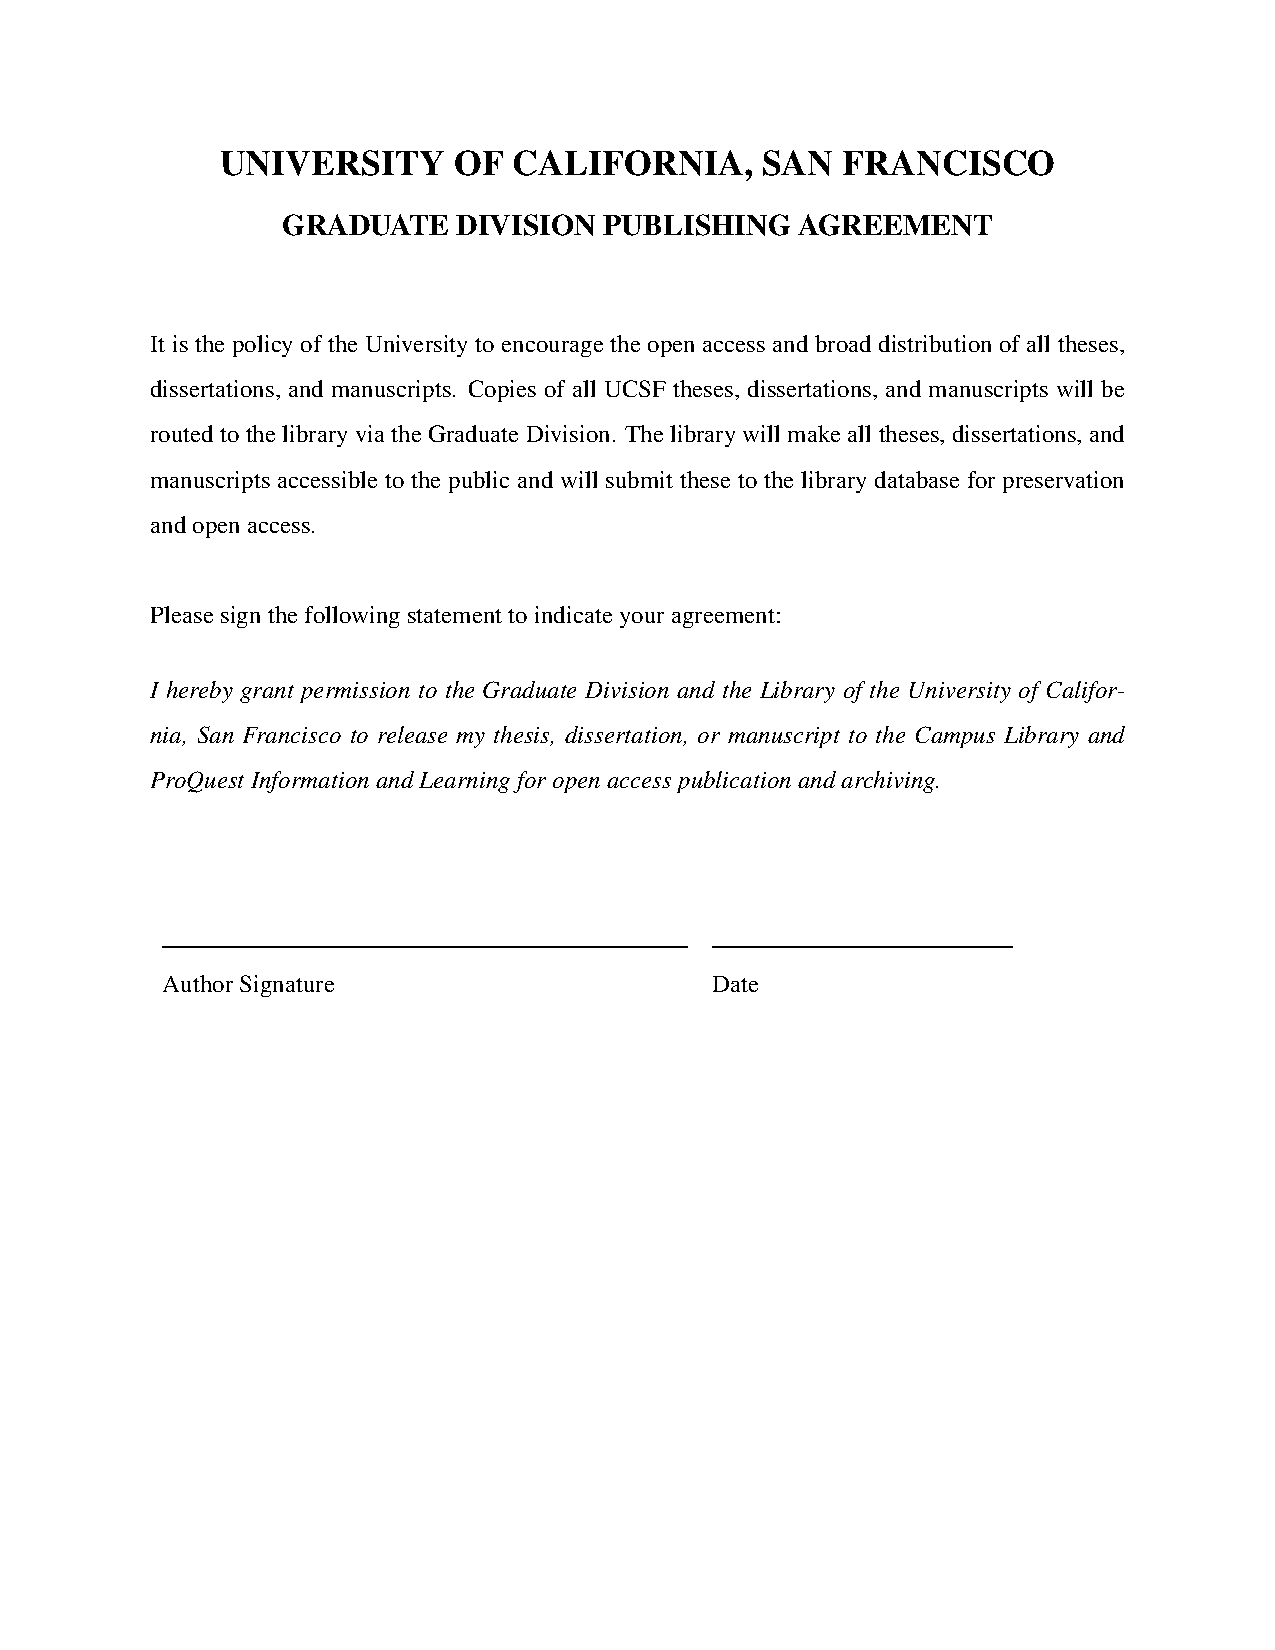
\includepdf[pages={1}, pagecommand={\thispagestyle{fancy}}]{publishing_agreement.pdf}

\end{document}
